\documentclass[crop,tikz]{standalone}% 'crop' is the default for v1.0, before it was 'preview'
\usepackage{physics}
\usetikzlibrary{positioning,shapes.geometric,decorations.pathreplacing,arrows.meta}
\begin{document}
\tikzset{meter/.append style={draw, inner sep=10, rectangle, font=\vphantom{A}, minimum width=30, line width=.8,
 path picture={\draw[black] ([shift={(.1,.3)}]path picture bounding box.south west) to[bend left=50] ([shift={(-.1,.3)}]path picture bounding box.south east);\draw[black,-latex] ([shift={(0,.1)}]path picture bounding box.south) -- ([shift={(.3,-.1)}]path picture bounding box.north);}}}

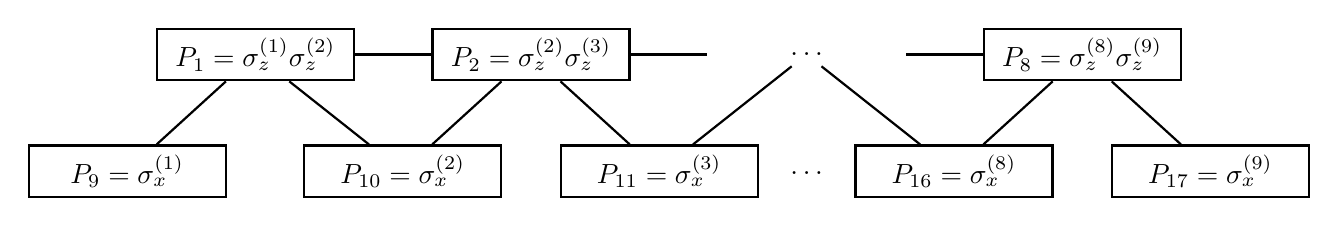
\begin{tikzpicture}[node distance={35mm}, thick, main/.style = {draw, rectangle,minimum width=2.5cm}
    ] 
\node[main] (0) {$P_1=\sigma_z^{(1)} \sigma_z^{(2)}$}; 
\node[main] (1) [right of=0] {$P_2=\sigma_z^{(2)} \sigma_z^{(3)}$};
\node (2) [right of=1, minimum width=2.5cm, rectangle] {$\ldots$};
\node[main] (3) [right of=2] {$P_8=\sigma_z^{(8)} \sigma_z^{(9)}$};
\node[main] (4) [below left=8mm and -9mm of 0] {$P_9=\sigma_x^{(1)}$};
\node[main] (5) [below left=8mm and -9mm of 1] {$P_{10}=\sigma_x^{(2)}$};
\node[main] (6) [below right=8mm and -9mm of 1] {$P_{11}=\sigma_x^{(3)}$};
\node (7) [below=12mm of 2, minimum width=2.5cm, rectangle] {$\ldots$};
\node[main] (8) [below left=8mm and -9mm of 3] {$P_{16}=\sigma_x^{(8)}$};
\node[main] (9) [below right=8mm and -9mm of 3] {$P_{17}=\sigma_x^{(9)}$};

\draw[-] (0) -- (1);
\draw[-] (1) -- (2);
\draw[-] (2) -- (3);
\draw[-] (0) -- (4);
\draw[-] (0) -- (5);
\draw[-] (1) -- (5);
\draw[-] (1) -- (6);
\draw[-] (2) -- (6);
\draw[-] (2) -- (8);
\draw[-] (3) -- (8);
\draw[-] (3) -- (9);

\end{tikzpicture} 
\end{document}
